% ft-14-Fundamental.tex

\documentclass[xcolor=dvipsnames]{beamer}

\usepackage{cancel}
\renewcommand{\CancelColor}{\color{red}}
\usepackage{graphicx}
\usepackage{wrapfig}
\usepackage{colortbl}
\usepackage{color}
\usepackage{alltt}
\renewcommand*{\thefootnote}{\fnsymbol{footnote}}
\definecolor{myblue}{rgb}{0.8,0.85,1}

\mode<presentation>
{
  \usetheme{Warsaw}
  \setbeamercovered{transparent}
}
% \usecolortheme[named=OliveGreen]{structure}
\setbeamertemplate{navigation symbols}{} 
\setbeamertemplate{blocks}[rounded][shadow=true] 

% this is for overlaying math symbols, see https://tex.stackexchange.com/questions/12895/overlay-symbol-with-another
\def\qeq{\mathrel{%
    \mathchoice{\QEQ}{\QEQ}{\scriptsize\QEQ}{\tiny\QEQ}%
}}
\def\QEQ{{%
    \setbox0\hbox{$\longrightarrow$}%
    \rlap{\hbox to \wd0{\hss/\hss}}\box0
  }}

\newcounter{expls}
\setcounter{expls}{0}
\newcommand{\beispiel}[1]{\refstepcounter{expls}\textbf{Example \arabic{expls}: #1.}}

\newcounter{exercise}
\setcounter{exercise}{0}
\newcommand{\ubung}[0]{\refstepcounter{exercise}\textbf{Exercise \arabic{exercise}: }}

\newif\ifBCITCourse
\BCITCoursetrue
% \BCITCoursefalse
\newif\ifWhichCourse
\WhichCoursetrue
% \WhichCoursefalse
\ifBCITCourse
\ifWhichCourse
\newcommand{\CourseName}{Technical Mathematics for Food Technology}
\newcommand{\CourseNumber}{MATH 1441}
\newcommand{\CourseInst}{BCIT}
\else
\newcommand{\CourseName}{Technical Mathematics for Geomatics}
\newcommand{\CourseNumber}{MATH 1511}
\newcommand{\CourseInst}{BCIT}
\fi
\else
\newcommand{\CourseName}{Philosophy and Literature}
\newcommand{\CourseNumber}{PHIL 375}
\newcommand{\CourseInst}{UBC}
\fi

\title{Fundamental Theorem of Calculus}
\subtitle{{\CourseNumber}, BCIT}

\author{\CourseName}

\date{November 28, 2017}

\begin{document}

\begin{frame}
  \titlepage
\end{frame}

\begin{frame}
  \frametitle{Antiderivatives}
Remember these two problems that we wanted to solve when we started
with calculus:
  \begin{figure}[h]
    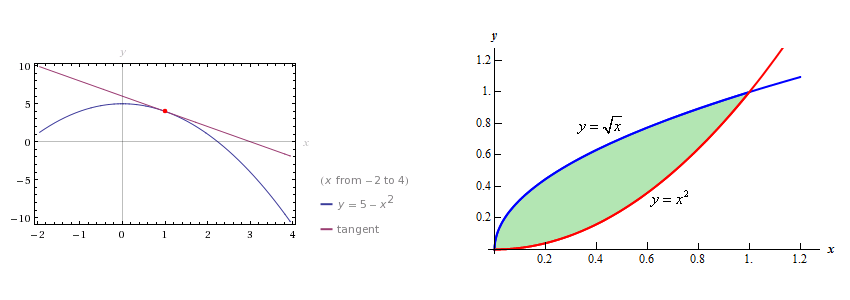
\includegraphics[scale=.35]{./regiontangent.png}
  \end{figure}
We have solved the problem on the left. Now it is time to solve the
problem on the right. For areas under a curve, we need
antiderivatives. The antiderivative $F(x)$ of a function $f(x)$ is the
function for which $F'(x)=f(x)$. 
\end{frame}

\begin{frame}
  \frametitle{Differential Equations}
Differential equations are like regular equations except that the
unknown is a function, not a variable. Remember that
\begin{equation}
  \label{eq:aiceiphe}
  dy=f'(x)\,dx\mbox{, therefore }f'(x)=\frac{dy}{dx}
\end{equation}
Now consider this differential equation,
\begin{equation}
  \label{eq:pheiwaot}
  \frac{dy}{dx}=f(x)
\end{equation}
This is an ODE, an \alert{ordinary differential equation}. 
\end{frame}

\begin{frame}
  \frametitle{Differential Equations}
\begin{equation}
  \label{eq:ahngohto}
  \frac{dy}{dx}=f(x)
\end{equation}
This is an ODE, an \alert{ordinary differential equation}. Any
function
\begin{equation}
  \label{eq:ogheigha}
  f(x)=e^{x}+C,C\in\mathbb{R}
\end{equation}
would solve it. Often, an \alert{initial condition} is provided to
make the solution unique. Therefore, the solution to the differential
equation
\begin{equation}
  \label{eq:joogeipo}
  \frac{dy}{dx}=f(x)
\end{equation}
with initial condition $f(0)=1$ is $f(x)=e^{x}$.
\end{frame}

\begin{frame}
  \frametitle{Differential Equations}
Antiderivatives are solutions to special differential equations. For
example, the antiderivative of $f(x)=6x$ is the solution to the
differential equation
\begin{equation}
  \label{eq:xoozazui}
  \frac{dy}{dx}=6x
\end{equation}
With an initial condition, the solution to this equation may be
unique.
\end{frame}

\begin{frame}
  \frametitle{Rules for Finding Antiderivatives}
  Antiderivatives are not unique. If $F(x)$ is an antiderivative for
  $f(x)$, then $F(x)+c$ is an antiderivative as well, where $c$ is any
  real number. In the following, we will use the notation $F(x)$ for
  one arbitrary antiderivative. There are many rules for finding
  antiderivatives called \emph{table of integrals}. Here are a few.
  \begin{block}{Rule 1}
    If you find a function $g(x)$ for which $g'(x)=f(x)$, then
    $F(x)=g(x)+c$.
  \end{block}
  Exercise: show that the function $g(x)$ is an antiderivative of
  $f(x)=(x^{3}+3)^{6}(3x^{2})$.
  \begin{equation}
    \label{eq:eiyahcei}
    g(x)=\frac{(x^{3}+3)^{7}}{7}
  \end{equation}
\end{frame}

\begin{frame}
  \frametitle{More Rules for Finding Antiderivatives I}
  \begin{block}{Rule 2}
    If $F(x)$ is an antiderivative for $f(x)$, then $aF(x)$ is an
    antiderivative for $af(x)$, where $a$ is a constant.
  \end{block}
\end{frame}

\begin{frame}
  \frametitle{More Rules for Finding Antiderivatives II}
  \begin{block}{Rule 3}
    If $F_{1}(x)$ is an antiderivative for $f_{1}(x)$ and $F_{2}(x)$
    is an antiderivative for $f_{2}(x)$, then $F_{1}(x)+F_{2}(x)$ is
    an antiderivative for $f_{1}(x)+f_{2}(x)$.
  \end{block}
\end{frame}

\begin{frame}
  \frametitle{More Rules for Finding Antiderivatives III}
  \begin{block}{Rule 4}
    If $f(x)=x^{n}$ and $n\neq{}-1$, then $F(x)=\frac{x^{n+1}}{n+1}$
    is an antiderivative of $f(x)$.
  \end{block}
Exercise: Find an antiderivative of $f(x)=1/x$. The answer is not
quite what you would expect (but very close). 
\end{frame}

\begin{frame}
  \frametitle{Summary}
Here is a table of antiderivatives, where $F$ is an antiderivative of
$f$ and $G$ is an antiderivative of $g$.

\medskip

\begin{tabular}{|l|l|}\hline
  $cf(x)$ & $cF(x)$ \\ \hline
  $f(x)+g(x)$ & $F(x)+G(x)$ \\ \hline
  $x^{n}$ with $n\neq{}-1$ & $\displaystyle \frac{x^{n+1}}{n+1}$ \\ \hline
  $\displaystyle \frac{1}{x}$ & $\ln\vert{}x\vert$ \\ \hline
  $e^{x}$ & $e^{x}$ \\ \hline
  $\cos{}x$ & $\sin{}x$ \\ \hline
  $\sin{}x$ & $-\cos{}x$ \\ \hline
  $\sec^{2}x$ & $\tan{}x$ \\ \hline
  $\sec{}x\tan{}x$ & $\sec{}x$ \\ \hline
  $\displaystyle \frac{1}{\sqrt{1-x^{2}}}$ & $\arcsin{}x$ \\ \hline
  $\displaystyle \frac{1}{1+x^{2}}$ & $\arctan{}x$ \\ \hline
\end{tabular}
\end{frame}

\begin{frame}
  \frametitle{Integration}
  The process of finding a derivative is called differentiation. The
  process of finding an antiderivative is called \alert{integration}.
  Instead of the symbol `prime' ($f'(x)$) for differentiation we use
  the sign $\int$ for integration. The symbol $\int$ stands for the
  word `sum' because we take the limit of a sum of areas in order to
  find the area under a curve.
\begin{equation}
  \label{eq:muixutoh}
  \int{}f(x)\,dx=F(x)+c
\end{equation}
The differential helps to identify which letter is the variable for
the function (there may be other letters that are just constants), for
example
\begin{equation}
  \label{eq:eighooko}
  \int{}ax^{2}\,dx=\frac{ax^{3}}{3}+c
\end{equation}
\begin{equation}
  \label{eq:ungiumah}
  \int{}ax^{2}\,da=\frac{a^{2}x^{2}}{2}+c
\end{equation}
\end{frame}

\begin{frame}
  \frametitle{Integration Exercises I}
Find the following \alert{indefinite integrals} (another expression
for antiderivatives). 
\begin{equation}
  \label{eq:eevoomoh}
  \int{}6\,dx
\end{equation}
\begin{equation}
  \label{eq:eohauthu}
  \int{}-2\,dx
\end{equation}
\begin{equation}
  \label{eq:heizieta}
  \int{}8x^{4}\,dx
\end{equation}
\begin{equation}
  \label{eq:zohjieph}
  \int{}\pi{}x^{3}\,dx
\end{equation}
\begin{equation}
  \label{eq:oodaelad}
  \int{}\left(x^{3}+7-2x^{2}\right)\,dx
\end{equation}
\begin{equation}
  \label{eq:eeshooyo}
  \int{}\sqrt{x}\,dx
\end{equation}
\begin{equation}
  \label{eq:uafievai}
  \int{}\frac{7}{2}x^{\frac{5}{2}}\,dx
\end{equation}
\end{frame}

\begin{frame}
  \frametitle{Integration Exercises II}
Find the following \alert{indefinite integrals} (another expression
for antiderivatives). 
\begin{equation}
  \label{eq:igheivei}
  \int{}9\sqrt[5]{2x}\,dx
\end{equation}
\begin{equation}
  \label{eq:akahheju}
  \int{}\frac{3}{x^{3}}\,dx
\end{equation}
\begin{equation}
  \label{eq:zeifahce}
  \int{}\frac{7}{\sqrt[3]{x}}\,dx
\end{equation}
\begin{equation}
  \label{eq:afahthud}
  \int{}\sqrt{x}\left(3x-2\right)\,dx
\end{equation}
\begin{equation}
  \label{eq:desheiga}
  \int{}\left(x+1\right)^{2}\,dx
\end{equation}
\begin{equation}
  \label{eq:oongaiqu}
  \int{}\frac{4x^{2}-2\sqrt{x}}{x}\,dx
\end{equation}
\begin{equation}
  \label{eq:ahxiequo}
  \int{}\frac{x^{3}+2x^{2}-3x-6}{x+2}\,dx
\end{equation}
\end{frame}

\begin{frame}
  \frametitle{Definite Integrals I}
Evaluating an integral at a point doesn't give us anything
particularly meaningful.
\begin{equation}
  \label{eq:beavaika}
  \int{}x^{2}\,dx=\frac{x^{3}}{3}+c
\end{equation}
\begin{equation}
  \label{eq:paeshohz}
  \left.\int{}x^{2}\,dx\right\vert_{x=6}=\frac{6^{3}}{3}+c=72+c
\end{equation}
However, if we subtract one evaluated integral from another, we get a number.
\begin{equation}
  \label{eq:phiasohm}
  \left.\int{}x^{2}\,dx\right\vert_{x=6}-\left.\int{}x^{2}\,dx\right\vert_{x=3}=\frac{6^{3}}{3}+c-\left(\frac{3^{3}}{3}+c\right)=72-9=63\notag
\end{equation}
\end{frame}

\begin{frame}
  \frametitle{Definite Integrals II}
We call this difference between evaluated integrals \alert{definite
  integral}. The notation is
\begin{equation}
  \label{eq:yooxiefi}
  \int_{3}^{6}x^{2}\,dx=\left.\int{}x^{2}\,dx\right\vert_{x=6}-\left.\int{}x^{2}\,dx\right\vert_{x=3}=63\notag
\end{equation}
\end{frame}

\begin{frame}
  \frametitle{Definite Integrals Exercises}
Evaluate each definite integral.
\begin{equation}
  \label{eq:ufaetohm}
  \int_{1}^{2}x\,dx\hspace{1in}  \int_{-2}^{2}x^{2}\,dx
\end{equation}
\begin{equation}
  \label{eq:vahyooyi}
  \int_{1}^{3}7x^{2}\,dx\hspace{1in}  \int_{-2}^{2}3s^{4}\,ds
\end{equation}
\begin{equation}
  \label{eq:wohbuxoo}
  \int_{0}^{4}(x^{2}+2x)\,dx\hspace{1in}  \int_{1}^{e}\frac{1}{x}\,dx
\end{equation}
\begin{equation}
  \label{eq:ohgooquu}
  \int_{5}^{10}\sqrt{x}\,dx\hspace{1in}\int_{1}^{4}\frac{2+x^{2}}{\sqrt{x}}\,dx
\end{equation}
\begin{equation}
  \label{eq:yoocaitu}
  \int_{-1}^{2}(3u-2)(u+1)\,du\hspace{1in}\int_{\frac{\pi}{6}}^{\pi}\sin\vartheta{}\,d\vartheta
\end{equation}
\end{frame}

\begin{frame}
  \frametitle{Fundamental Theorem of Calculus I}
  It turns out that the definite integral $\int_{a}^{b}f(x)\,dx$ gives
  you the area under the curve $y=f(x)$ between $a$ and $b$. This area
  can be approximated by a series of rectangles.
\begin{figure}[h]
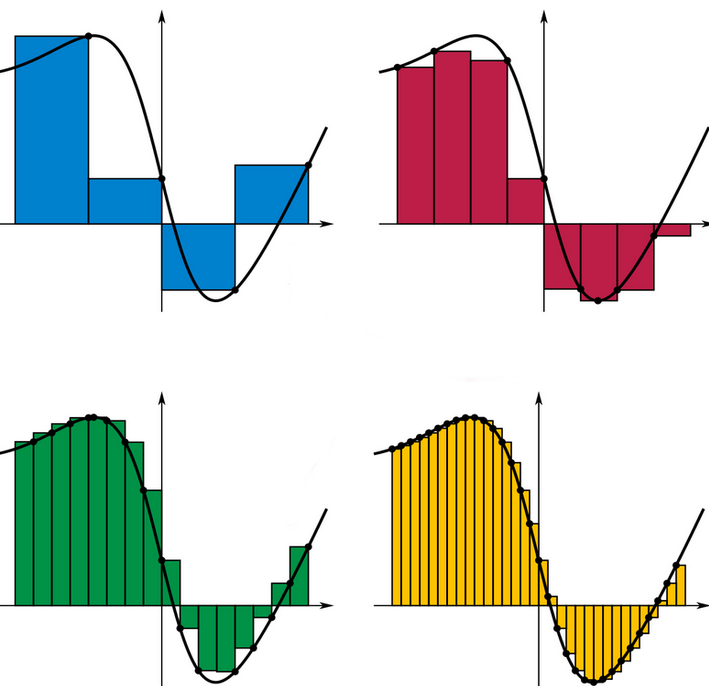
\includegraphics[scale=.3]{./ftoc-02.png}
\end{figure}
\end{frame}

\begin{frame}
  \frametitle{Fundamental Theorem of Calculus II}
Let's assume our function is positive between $a$ and $b$, so
$f(x)\geq{}0$ for $a\leq{}x\leq{}b$. Let $F$ be an antiderivative of
$f$. Here is the \alert{mean value theorem}, a theorem we need to
assume without proof: between two arguments $r$ and $s$ we can always
find a point $q$ such that the slope of the secant line between $F(r)$
and $F(s)$ equals the slope of the tangent line at $F(q)$, so
\begin{equation}
  \label{eq:zahrahsi}
  F'(q)=\frac{F(s)-F(r)}{s-r}\mbox{ (MVT)}\notag
\end{equation}
\begin{figure}[h]
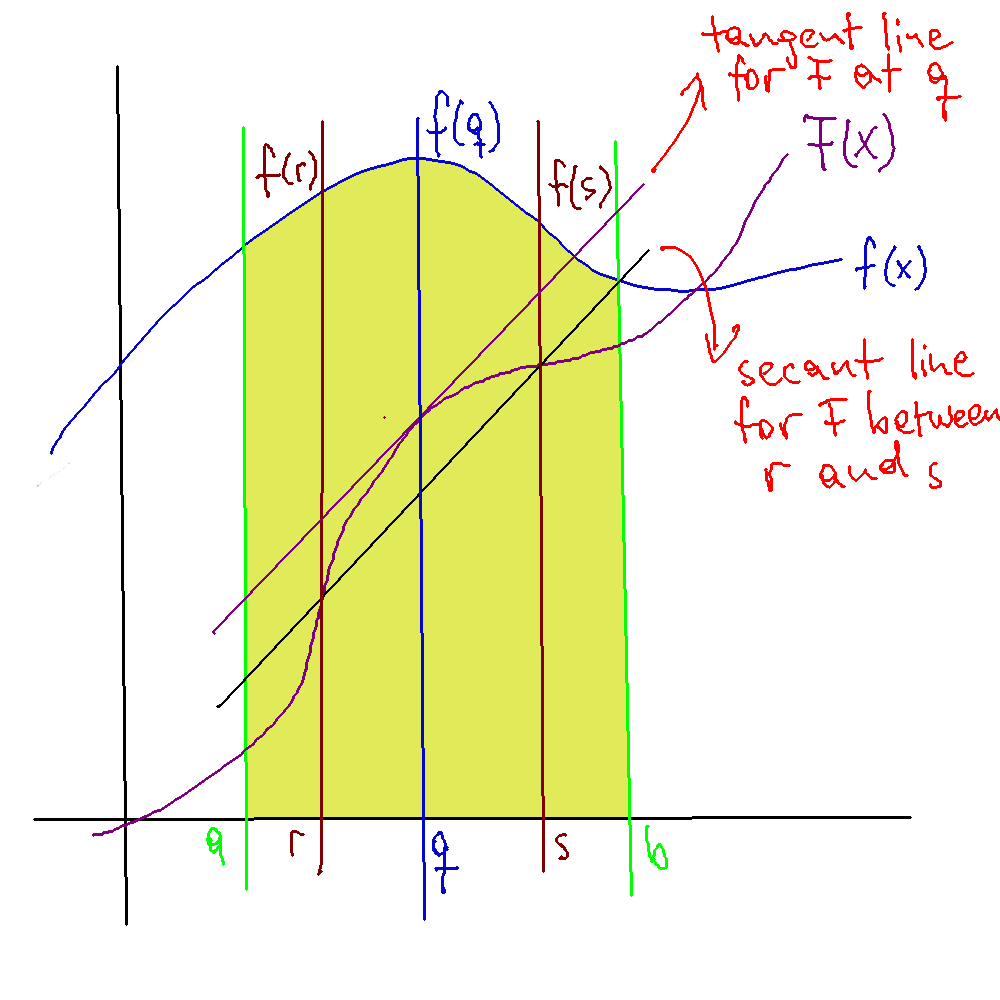
\includegraphics[scale=.13]{./ftoc-01.png}
\end{figure}
\end{frame}

\begin{frame}
  \frametitle{Fundamental Theorem of Calculus III}
Now divide the interval from $a$ to $b$ (the notation for this
interval is $[a,b]$) into $n$ intervals that are of equal length. For
this, we need intermediate points
$a=x_{0},x_{1},x_{2},\ldots,x_{n-1},x_{n}=b$. The approximate area
under the curve between $a$ and $b$ is
\begin{equation}
  \label{eq:eikaidei}
  A\approx\frac{x_{1}-a}{n}f(x_{1}^{*})+\frac{x_{2}-x_{1}}{n}f(x_{2}^{*})+\ldots+\frac{b-x_{n-1}}{n}f(x_{n}^{*})
\end{equation}
where $x_{1}^{*}$ is some point in the first interval and so on.
Notice that the fractions all equal $(b-a)/n$ because the intervals
are all of equal length. Therefore
\begin{equation}
  \label{eq:pukaepha}
  A=\lim_{n\rightarrow\infty}\frac{b-a}{n}\left(f(x_{1}^{*})+\ldots+f(x_{n}^{*})\right)
\end{equation}
\end{frame}

\begin{frame}
  \frametitle{Fundamental Theorem of Calculus IV}
Now choose $x_{1}^{*}$ such that 
\begin{equation}
  \label{eq:bicochoh}
  f(x_{1}^{*})=F'(x_{1}^{*})=\frac{F(x_{1})-F(x_{0})}{x_{1}-x_{0}}
\end{equation}
and so on with $x_{2}^{*},x_{3}^{*},\ldots,x_{n}^{*}$. Then
\begin{equation}
  \label{eq:chabahxo}
  A=\lim_{n\rightarrow\infty}\frac{b-a}{n}\left(\frac{F(x_{1})-F(x_{0})}{x_{1}-x_{0}}+\ldots+\frac{F(x_{n})-F(x_{n-1})}{x_{n}-x_{n-1}}\right)
\end{equation}
Note that $x_{i}-x_{i-1}$ (where $i$ is any number between 1 and $n$)
is again just the length of the intervals $(b-a)/n$. After appropriate
simplification,
\begin{equation}
  \label{eq:ovooleek}
  A=F(b)-F(a)=\int_{a}^{b}f(x)\,dx
\end{equation}
\end{frame}

\begin{frame}
  \frametitle{Fundamental Theorem of Calculus V}
Here are two different ways to express the Fundamental Theorem of
Calculus.
\begin{block}{The Fundamental Theorem of Calculus}
  Suppose $f$ is continuous on $[a,b]$.
  \begin{enumerate}
  \item If $g(x)=\int_{a}^{x}f(t)\,dt$, then $g'(x)=f(x)$.
  \item $\int_{a}^{b}f(x)\,dx=F(b)-F(a)$, where $F$ is any
    antiderivative of $f$, that is, $F'=f$.
  \end{enumerate}
\end{block}
Note that we need not require $a\leq{}b$. If the limits of integration
are unintuitively placed, you can rectify the situation by using 
\begin{equation}
  \label{eq:vichujai}
  \int_{b}^{a}f(x)\,dx=F(a)-F(b)=-(F(b)-F(a))=-\int_{a}^{b}f(x)\,dx\notag
\end{equation}
\end{frame}

\begin{frame}
  \frametitle{Fundamental Theorem of Calculus Exercises}
{\ubung} Find the area under the parabola
\begin{equation}
  \label{eq:veigheph}
  y=x^{2}
\end{equation}
from $0$ to $1$.
\end{frame}

\begin{frame}
  \frametitle{Negative Area}
Consider the following problem.
\begin{block}{}
Find the area under the curve $y=x^{2}-4$ between $x=1$ and $x=3$.
\end{block}
\begin{figure}[h]
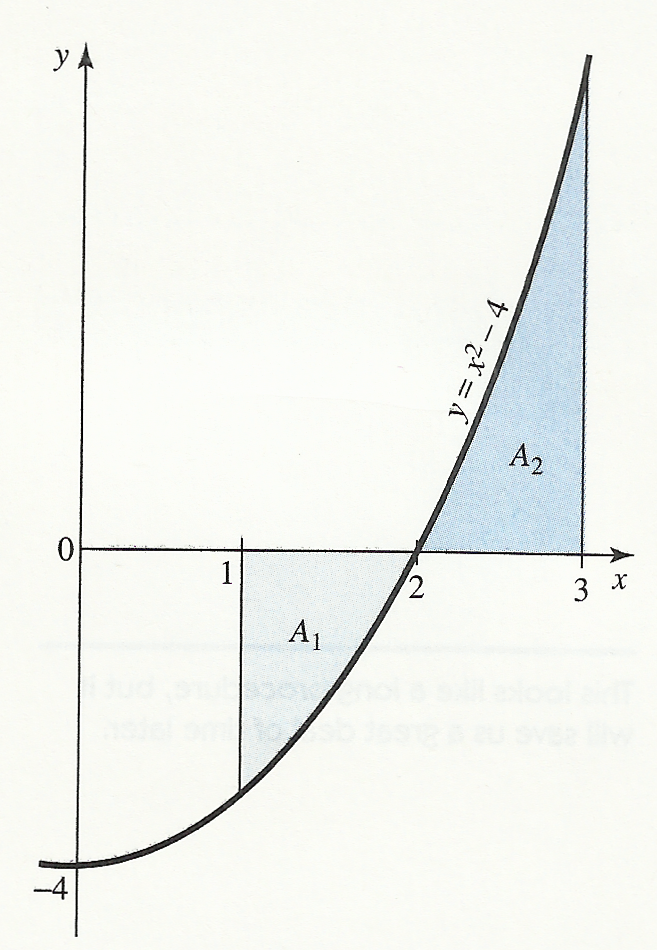
\includegraphics[scale=.6]{./negarea.png}
\end{figure}
\end{frame}

\begin{frame}
  \frametitle{Negative Area}
To solve this problem, find the $x$-intercept and treat the positive
and negative area separately. 
\begin{equation}
  \label{eq:aisohphu}
  \vert{}A_{1}\vert{}+\vert{}A_{2}\vert{}=-\int_{1}^{2}(x^{2}-4)\,dx+\int_{1}^{2}(x^{2}-4)\,dx=-\left(-\frac{5}{3}\right)+\frac{7}{3}=4\notag
\end{equation}
\end{frame}

\begin{frame}
  \frametitle{Integration by Substitution}
We know how to integrate the following functions
\begin{equation}
  \label{eq:deixugha}
  f_{1}(y)=y^{3}\mbox{ and }f_{2}(x)=2x+5
\end{equation}
but how do you integrate $f=f_{1}\circ{}f_{2}$, so
\begin{equation}
  \label{eq:eetusiil}
  f(x)=(2x+5)^{3}
\end{equation}
We use the method of \alert{substitution}. Write 
\begin{equation}
  \label{eq:ohshaoxe}
  y=2x+5
\end{equation}
The important part here is that the substitution changes the
differential and the limits.
\begin{equation}
  \label{eq:ushooxiu}
  dy=2dx\mbox{ and therefore }dx=\frac{1}{2}dy
\end{equation}
Therefore,
\begin{equation}
  \label{eq:olaihaxi}
  \int_{a}^{b}(2x+5)^{3}dx=\int_{2a+5}^{2b+5}y^{3}\cdot{}\frac{1}{2}dy
\end{equation}
\end{frame}

\begin{frame}
  \frametitle{Integration by Substitution Example}
Let's evaluate $\int_{0}^{4}x\sqrt{9+x^{2}}dx$. We will do this two
ways. For method 1, we find the indefinite integral of
$x\sqrt{9+x^{2}}$ and then use the limits $a=0,b=4$ to evaluate the
definite integral. For method 2, we proceed as on the previous slide
and change both differential and limits for the definite interval.
Here is method 1. Substitute $y=9+x^{2}$. Then, $dy=2xdx$, so 
\begin{equation}
  \label{eq:iachuejo}
  \frac{1}{2}dy=xdx
\end{equation}
Notice that we need the factor $x$ on the right-hand side in order to
make this integration work.
\begin{equation}
  \label{eq:diacheiv}
  \int{}x\sqrt{9+x^{2}}dx=\frac{1}{2}\int{}\sqrt{y}dy=\frac{1}{2}\cdot\frac{y^{\frac{3}{2}}}{\frac{3}{2}}
\end{equation}
\end{frame}

\begin{frame}
  \frametitle{Integration by Substitution Example}
Now reverse the substitution
\begin{equation}
  \label{eq:shaixeen}
\frac{1}{2}\cdot\frac{y^{\frac{3}{2}}}{\frac{3}{2}}=\frac{1}{3}(9+x^{2})^{\frac{3}{2}}
\end{equation}
and evaluate the definite integral
\begin{equation}
  \label{eq:eileevar}
\int_{0}^{4}x\sqrt{9+x^{2}}dx=\notag
\end{equation}
\begin{equation}
  \label{eq:lumuewah}
\left.\frac{1}{3}(9+x^{2})^{\frac{3}{2}}\right\vert_{x=4}-\left.\frac{1}{3}(9+x^{2})^{\frac{3}{2}}\right\vert_{x=0}=\frac{98}{3}
\end{equation}
\end{frame}

\begin{frame}
  \frametitle{Integration by Substitution Example}
Here is method 2.
\begin{equation}
  \label{eq:waethish}
  \int_{0}^{4}x\sqrt{9+x^{2}}dx=\frac{1}{2}\int_{9}^{25}\sqrt{y}dy=\notag
\end{equation}
\begin{equation}
  \label{eq:anguyaeh}
  \frac{1}{3}\left(\left.y^{\frac{3}{2}}\right\vert_{y=25}-\left.y^{\frac{3}{2}}\right\vert_{y=9}\right)=\frac{1}{3}(125-27)=\frac{98}{3}
\end{equation}
\end{frame}

\begin{frame}
  \frametitle{Exercises}
% These exercises and the previous material are from S.T. Tan, Calculus
% for the Managerial, Life, and Social Sciences, p447.
{\ubung} Evaluate the following definite integrals.
\begin{equation}
  \label{eq:mauphouw}
  \int_{0}^{2}x(x^{2}-1)^{3}dx\hspace{1in}\int_{0}^{1}x^{2}(2x^{3}-1)^{4}dx
\end{equation}
\begin{equation}
  \label{eq:pahteeth}
  \int_{0}^{1}x\sqrt{5x^{2}+4}dx\hspace{1in}\int_{1}^{3}x\sqrt{3x^{2}-2}dx
\end{equation}
\begin{equation}
  \label{eq:ceiquoor}
  \int_{0}^{2}x^{2}(x^{3}+1)^{\frac{3}{2}}dx\hspace{1in}\int_{1}^{5}(2x-1)^{\frac{5}{2}}dx
\end{equation}
\begin{equation}
  \label{eq:riweevie}
  \int_{0}^{1}\frac{1}{\sqrt{2x+1}}dx\hspace{1in}\int_{0}^{2}\frac{x}{\sqrt{x^{2}+5}}dx
\end{equation}
\end{frame}

\begin{frame}
  \frametitle{Exercises}
{\ubung} Evaluate the following definite integrals.
\begin{equation}
  \label{eq:aigighau}
  \int_{1}^{2}(2x+4)(x^{2}+4x-8)^{3}dx\hspace{1in}\int_{-1}^{1}x^{2}(x^{3}+1)^{4}dx
\end{equation}
\begin{equation}
  \label{eq:omixughu}
  \int_{0}^{2}xe^{x^{2}}dx\hspace{1in}\int_{0}^{1}e^{-1}dx
\end{equation}
\begin{equation}
  \label{eq:baemixeg}
  \int_{3}^{6}\frac{2}{x-2}dx\hspace{1in}\int_{0}^{1}\frac{e^{x}}{1+e^{x}}dx
\end{equation}
\begin{equation}
  \label{eq:aeteepah}
  \int_{0}^{1}\frac{x}{1+2x^{2}}dx\hspace{1in}\int_{1}^{2}\frac{\ln{}x}{x}dx
\end{equation}
\end{frame}

\begin{frame}
  \frametitle{Negative Area Exercise}
  {\ubung} Find the area between the curve $y=2(x-5)^{2}-2$ and the
  $x$-axis between $x=3$ and $x=7$.
\begin{figure}[h]
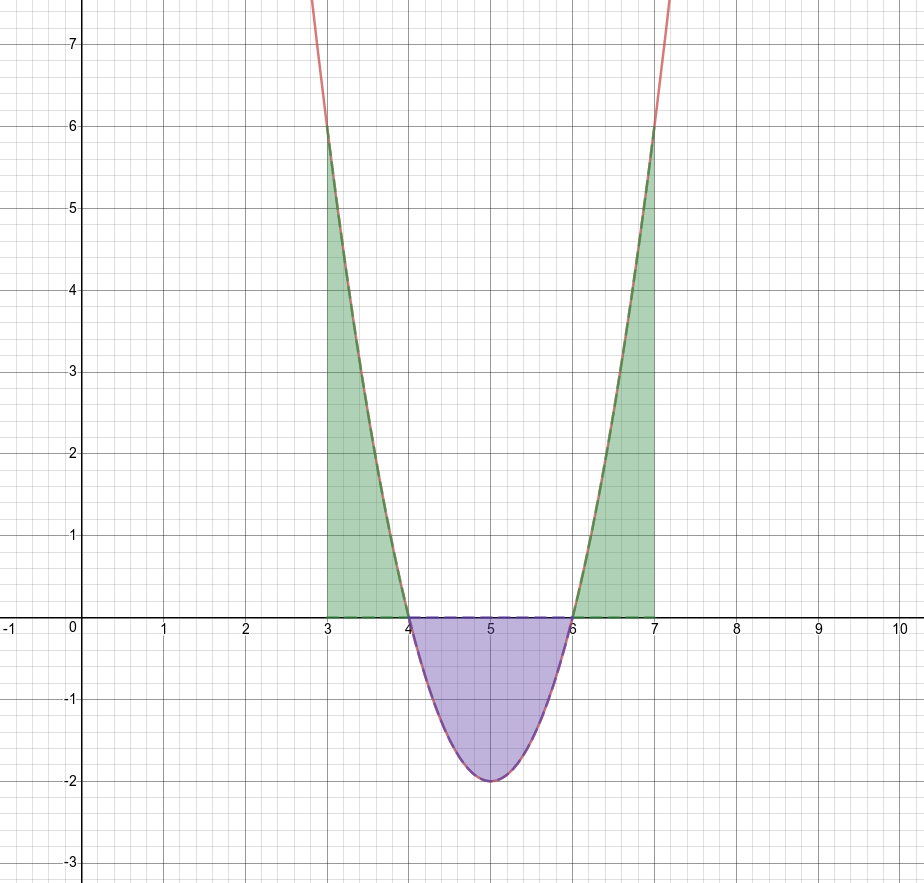
\includegraphics[scale=.2]{./NegativeArea.png}
\end{figure}
\end{frame}

\begin{frame}
  \frametitle{Area Between Curves}
  {\ubung} Find the area bounded by the curves $f(x)$ and $g(x)$.
\begin{figure}[h]
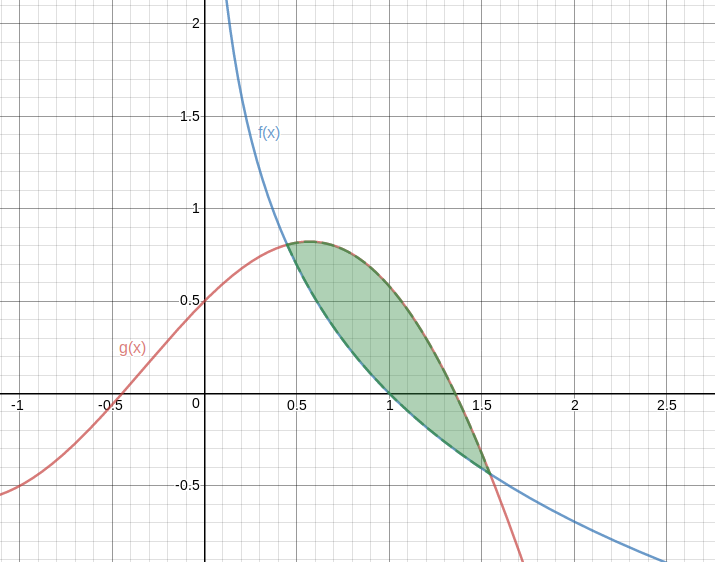
\includegraphics[scale=.15]{./areabetwcurs.png}
\end{figure}
To find this area, solve for the two solutions $x_{1},x_{2}$ of 
\begin{equation}
  \label{eq:aikooyae}
  f(x)=g(x)
\end{equation}
(you may have to use Newton's method) and then integrate
\begin{equation}
  \label{eq:upofahma}
  A=\int_{x_{1}}^{x_{2}}\left(g(x)-f(x)\right)\,dx
\end{equation}
\end{frame}

\begin{frame}
  \frametitle{Area Between Curves Exercise}
{\ubung} Find the area of the region enclosed by the parabola
$y=2-x^{2}$ and the line $y=-x$. 
\begin{figure}[h]
  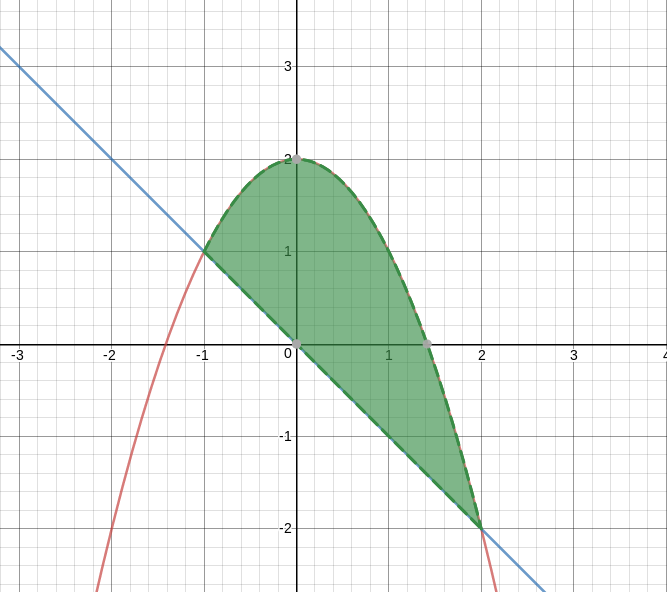
\includegraphics[scale=0.2]{./areabc.png}
\end{figure}
\end{frame}

\begin{frame}
  \frametitle{End of Lesson}
Next Lesson: That's all, folks! See you next year!
\end{frame}

\end{document}

